\newpage

{\centering
\normal
\textbf{ОСНОВНАЯ ЧАСТЬ}\par
}
\addcontentsline{toc}{chapter}{ОСНОВНАЯ ЧАСТЬ}

\customsection{Как пользоваться шаблоном}

\customsubsection{Че по содержанию диплома}

В целом шаблон довольно понятный.
Где формат строго регламентирован стоят TODO'шки, их нужно заменить на ваш текст.
В остальном вы ограничены только вашей фантазией, но пара советов по структуре есть в пункте ~\ref{subsubsec:chapters}.

\customsubsubsection{Структура диплома в целом}
\begin{enumerate}
    \item ТИТУЛ (см.\ ~\ref{subsubsec:titul}) (\texttt{/extra/Title.pdf})
    \item РЕФЕРАТ (см.\ ~\ref{subsubsec:intro}) (\texttt{/chapters/introduction.tex})
    \item СОДЕРЖАНИЕ (см.\ ~\ref{subsubsec:intro}) (\texttt{/chapters/introduction.tex})
    \item ОБОЗНАЧЕНИЯ И СОКРАЩЕНИЯ (см.\ ~\ref{subsubsec:intro}) (\texttt{/chapters/introduction.tex})
    \item ВВЕДЕНИЕ (см.\ ~\ref{subsubsec:intro}) (\texttt{/chapters/introduction.tex})
    \item ОСНОВНАЯ ЧАСТЬ (см.\ ~\ref{subsubsec:chapters}) (\texttt{/chapters/chapter\_1.tex})
    \begin{itemize}
        \item Глава 1 (\texttt{/chapters/chapter\_1.tex})
        \item Глава 2 (\texttt{/chapters/chapter\_2.tex})
        \item \ldots
        \item Глава N (\texttt{/chapters/chapter\_N.tex})
    \end{itemize}
    \item ЗАКЛЮЧЕНИЕ (см.\ ~\ref{subsubsec:concl}) (\texttt{/chapters/conclusion.tex})
    \item СПИСОК ИСПОЛЬЗОВАННЫХ ИСТОЧНИКОВ И ЛИТЕРАТУРЫ (см.\ ~\ref{subsubsec:bibki})
    \item (опционально) ПРИЛОЖЕНИЕ А (\texttt{/chapters/appendix\_A.tex})
    \item (опционально) ПРИЛОЖЕНИЕ B (\texttt{/chapters/appendix\_B.tex})
\end{enumerate}

\customsubsubsection{Титул}\label{subsubsec:titul}
Есть несколько разных конфигураций руководителей, в зависимости от которых титулы будут отличаться:
\begin{itemize}
    \item Руководитель \textbf{(не доцент)} от УрФУ + Соруководитель \textbf{(доцент)} от Урфу — \href{https://docs.google.com/document/d/1IOgZB7tnBZlSC6jNtLQielXxP-NEtd9Aqqy75Bwn0ko}{шаблон}
    \item \textit{шаблонов для других конфигураций у меня пока что нет, если есть у вас — пишите в \href{https://t.me/pohotlivi_ded}{телегу}}
\end{itemize}

После того как сделаешь титул, скачиваешь его в PDF и кладешь в \texttt{/extra/Title.pdf}

\customsubsubsection{Реферат + Содержание + Глоссарий + Введение}\label{subsubsec:intro}
Кажется структура у всех +- одинаковая, поэтому в файле \texttt{./introduction.tex} заменяешь все TODO'шки под себя
Содержание генерируется само

\customsubsubsection{Главы}\label{subsubsec:chapters}
Этот пункт только для программистов, как должно быть у математиков не знаю :(

Тут, вроде как, строгих регламентов нет, но чтобы была цельная, логичная картина происходящего, логично организовать структуру так:
\begin{enumerate}
    \item Анализ того что ты собираешься делать: существующие решения, какие технологии применяют и т.п.
    \item Постановка задач
    \item Выбор технологий на основании анализа и построение архитектуры
    \item Далее выполнение задач, можно разбить на несколько глав
    \item \ldots
\end{enumerate}

\customsubsubsection{Заключение}\label{subsubsec:concl}
Тут в целом все по аналогии с введением, заменяем TODO'шки в файле \texttt{./conclusion.tex}.

\customsubsubsection{Список литературы}\label{subsubsec:bibki}
Ниже будет подробный пункт про то, как составить библиографию

\customsubsubsection{Приложения}\label{subsubsec:appl}
Прикладываем все что надо (и если надо) в файлы \texttt{./appendix\_A.tex} и \texttt{./appendix\_B.tex}

\newpage
\customsubsection{Как работать с источниками}
Все источники лежат в файле с бибками, он же \texttt{/biblio/bibliography.bib}\\
\textbf{!!Attention!! все кириллические символы в файле с бибками нужно заворачивать в \texttt{\{\textbackslash cyr Ну это по-русски, но все равно круто!\}}}

Но сначала надо найти источник, тут есть два стула:
\begin{enumerate}
    \item Электронный источник (доки, туториалы и т.п.)
    \item Статьи, книги и т.п.
\end{enumerate}
Алгоритмы работы с ними немного отличаются.

\customsubsubsection{Электронные источники}
Это всякие ссылки на документацию и т.п.
Для того, чтобы добавить электронный источник, нужно заполнить его по такому шаблону:

\codeblockfile[linerange={1-5},frame=single]{Шаблон бибок}{lst:bibki}{extra/bibki.txt}
И вставить в \texttt{/biblio/bibliography.bib}

\customsubsubsection{Статьи и книги}
Тут проще:
\begin{enumerate}
    \item Заходим на \href{https://scholar.google.com/}{scholar.google.com}
    \item В поиске ищем нужную статью
    \item Нажимаем кнопку \textbf{цитировать}
    \begin{figure}[H]
        \centering
        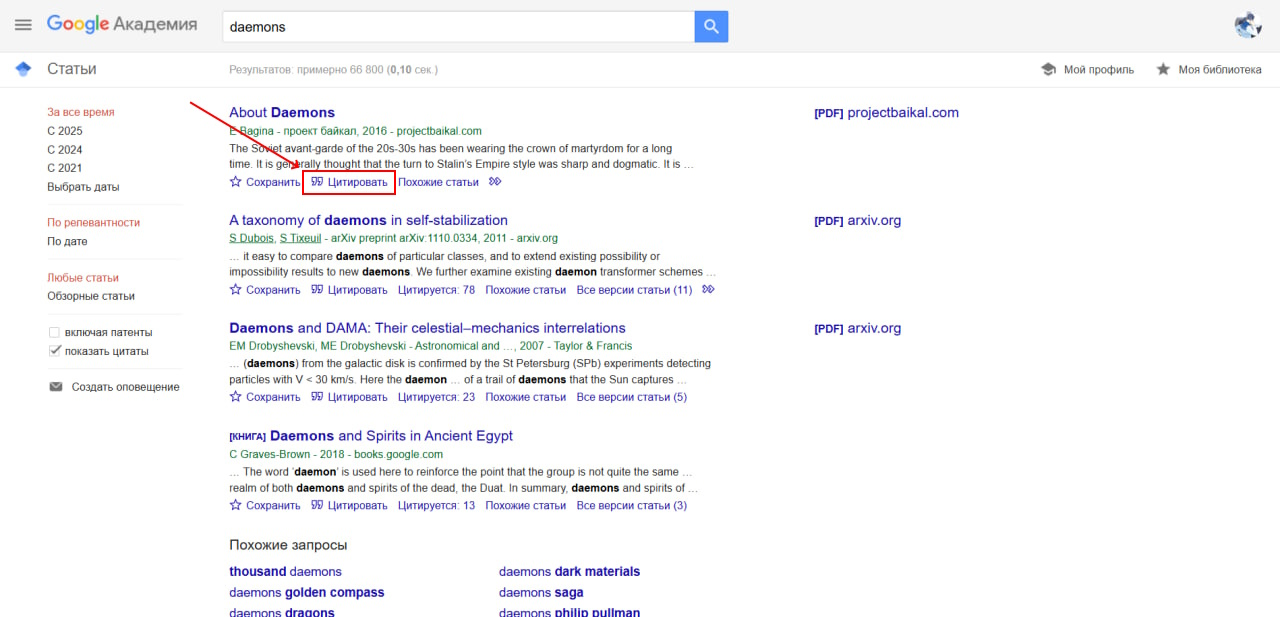
\includegraphics[width=150mm]{images/search}
        \caption{Поиск в Google Школяре}
        \label{fig:searhc}
    \end{figure}
    \item Нажимаем ссылку \textbf{BibTex}
    \begin{figure}[H]
        \centering
        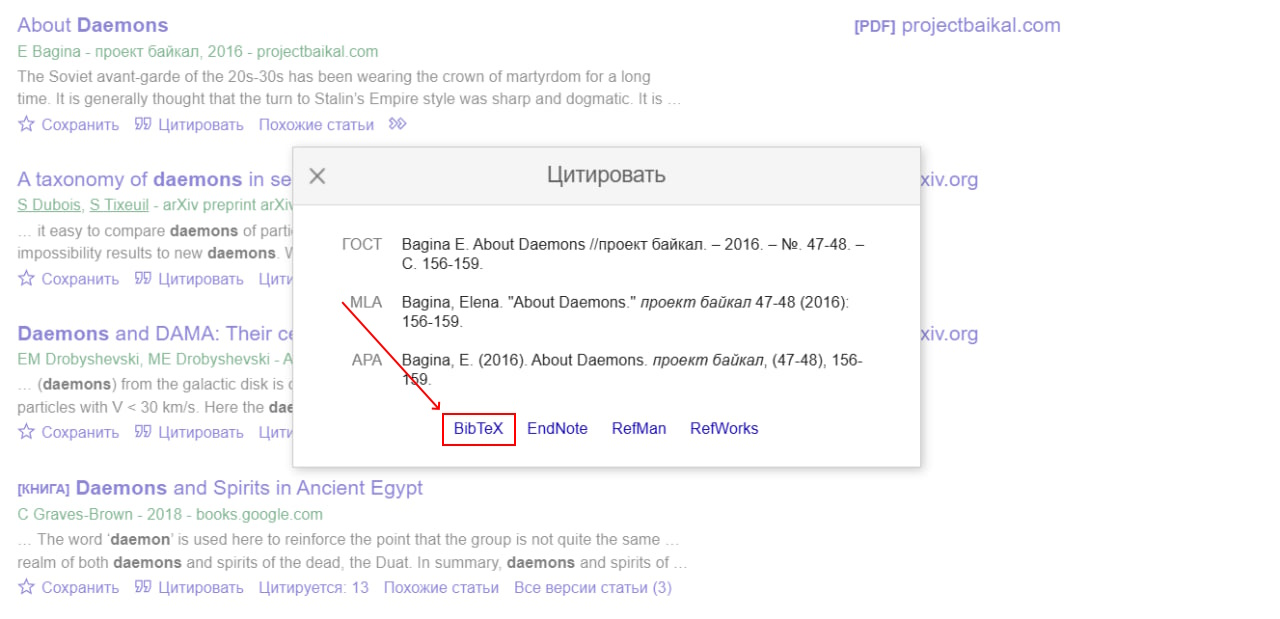
\includegraphics[width=150mm]{images/quote}
        \caption{Цитирование в Google Школяре}
        \label{fig:quote}
    \end{figure}
    \item Получаем что-то типа такого:
    \begin{figure}[H]
        \centering
        
\includegraphics[width=150mm]{images/bibtex}
        \caption{Готовая бибка}
        \label{fig:bibtex}
    \end{figure}
    \item вставляем в \texttt{/biblio/bibliography.bib}
\end{enumerate}

\customsubsubsection{А теперь цитируем}
В тексте можно сослаться так:
\begin{codeblockenv}{Прямой код}{lst:cite}
\begin{lstlisting}[language=Tex,frame=single]
Согласно ~\cite{docker} траляля ...\\
Согласно ~\cite{bagina2016daemons,dubois2011taxonomy}
\end{lstlisting}
\end{codeblockenv}
Результат:\\
Согласно ~\cite{docker} траляля ...\\
Согласно ~\cite{bagina2016daemons,dubois2011taxonomy} трампапам...

Также в настройках есть специальная строчка \texttt{\textbackslash nocite{*}}\\
Это нужно, чтобы источники, на которые нет ссылок в тексте, все равно отрисовывались в списке источников

\newpage
\customsubsection{Ну и как вставлять всякое}
\begin{table}[H]
    \caption{Пример вставки таблицы}\label{tab:table}
    \centering
    \begin{tabular}{|p{2.3cm}|p{2.0cm}|p{3cm}|p{1.5cm}|p{1.5cm}|p{1.5cm}|p{1.6cm}|} % Настройка ширин столбцов, | означает границы между столбцами
        \hline
        \textbf{Система} & \textbf{Источн.}     & \textbf{Фильтр}        & \textbf{Ключ. слова} & \textbf{Анали\-тика} & \textbf{API} & \textbf{Отказо\-устойч.} \\ \hline
        Brand Analytics  & СМИ, соц. сети       & Расшир. поиск          & Да                   & Да                   & Да           & Высок.                   \\ \hline
        YouScan          & Соцсети              & Интелл. фильтры        & Да                   & Да                   & Да           & Да                       \\ \hline
        Semantic Force   & Новости, соц. сети   & Контекст. анализ       & Да                   & Да                   & Да           & Не указано               \\ \hline
        Medialogia       & ТВ, радио, СМИ       & Огранич. функции       & Нет                  & Да                   & Да           & Да                       \\ \hline
        IQBuzz           & Соц. сети, форумы    & Поиск по ключ. словам  & Да                   & Огр.                 & Да           & Нет данных               \\ \hline
        Talkwalker       & СМИ, соц. сети       & Многоуровн. фильтрация & Да                   & Да                   & Да           & Да                       \\ \hline
    \end{tabular}
\end{table}

\begin{figure}[H]
    \centering
    
\includegraphics[width=150mm]{images/lev}
    \caption{Пример вставки рисунка}
    \label{fig:lev}
\end{figure}

\codeblockfile[linerange={1-5},frame=single]{Пример вставки кода из файла}{lst:bubku}{extra/bibki.txt} % linerange - строки которые надо взять; lst:bubku - лейбл для ссылок

\begin{codeblockenv}{Пример вставки кода текстом}{lst:cite}
    \begin{lstlisting}[language=Python,frame=single]
for i in range(1337):
    if (i % 69 == 0):
        print(228)
    \end{lstlisting}
\end{codeblockenv}

\customsubsection{Компиляция}
Про запуск и тп подробно расписано в \texttt{readme}

\customsubsection{Связь}
Если ты нашел ошибку, неправильное форматирование или просто появились вопросы, смело пиши в телегу \href{https://t.me/pohotlivi_ded}{@pohotlivi_ded} или можно сразу контрибутить в gitnub
